\usepackage[authoryear,round]{natbib}
\usepackage{multirow}

\newcommand{\sheetnum}{%
	08
}
%\setcounter{section}{\sheetnum-3}
\newcommand{\tutorialtitle}{%
    Class Imbalance and RBF-Networks
}
\newcommand{\tutorialtitleshort}{%
	RBF
}
% for slides
\subtitle{\sheetnum \tutorialtitle}

%\maxdeadcycles=1000 % Workaround for ! Output loop---100 consecutive dead cycles because of too many figures

% The following use of algroithms does not work well with the notes:
%
%
%
%
% instead use the following for your algorithms:
%
%\begin{figure}[!t]
%\removelatexerror
%\begin{algorithm}[H]
    % your algo here
    %\label{alg:algolabel}
    %\caption{algocaption}
%\end{algorithm}
%\end{figure}
%\begin{algorithm}
% Below is the definition for the command \removelatexerror:
\makeatletter
\newcommand{\removelatexerror}{\let\@latex@error\@gobble}
\makeatother

\begin{document} %%%%%%%%%%%%%%%%%%%%%%%%%%%%%%%%%%%%%%%%%%%%%%%%%%%%%%%

\sheet{\sheetnum}{\tutorialtitleshort}

\ttopic{\tutorialtitle}

\columnratio{0.2,0.8}\textbf{}
\begin{paracol}{2}
%\setlength{\columnseprule}{0.1pt}
%\setlength{\columnsep}{5em}

\begin{rightcolumn}

% notes version will ignore it
\begin{frame}
\titlepage
\end{frame}

\begin{frame}
\tableofcontents
\end{frame}

\mode<all>
\section{Dealing with imbalanced data}

\subsection{Motivation}

\begin{frame}\frametitle{\subsecname}

\only<1>{
Proportion of class labels in the dataset is not uniform.
Not the same as ``easy vs. difficult'' classes. This is only about class frequency.
}

\slidesonly{\vspace{-5mm}}

\begin{figure}[ht]
     \centering
     \savebox{\imagebox}{
	 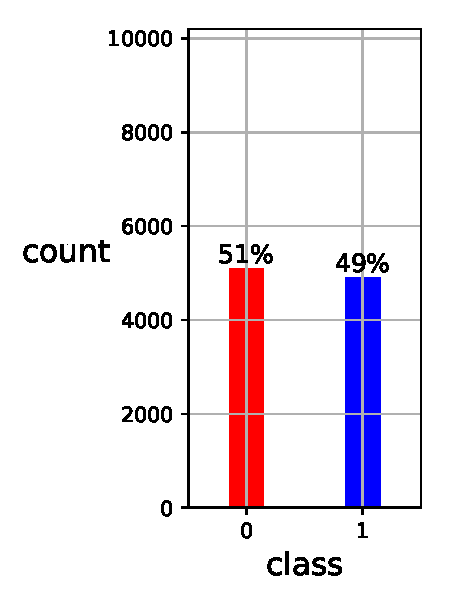
\includegraphics[width=0.28\textwidth]{img/hist_balanced}}%
     \begin{subfigure}[t]{0.28\textwidth}
         \centering
         \usebox{\imagebox}% Place largest image
         \caption{balanced $\approx 1:1$}
     \end{subfigure}
     \hspace{5mm}
     \begin{subfigure}[t]{0.28\textwidth}
         \centering
         \raisebox{\dimexpr.5\ht\imagebox-.5\height}{% Raise smaller image into place
         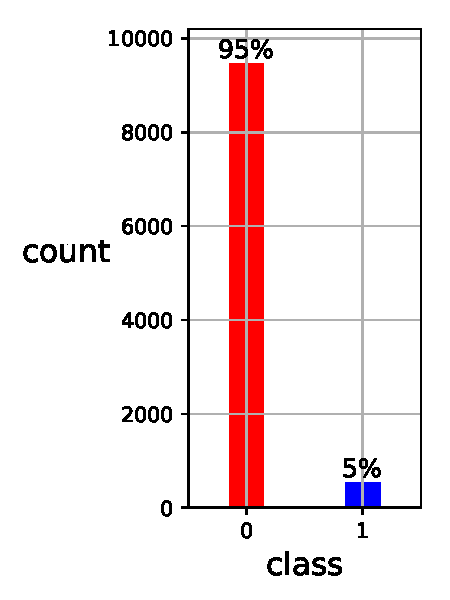
\includegraphics[width=0.99\textwidth]{img/hist_imbalanced}
         }
         \caption{highly unbalanced}
         \label{fig:linear}
     \end{subfigure}
\end{figure} 

\only<2>{     
A strong imbalance leads to the classifier learning a trivial solution that indeed minimizes the average cost over the training samples.
}
\only<2>{
\begin{equation}
E^T = \sum_{\alpha=1}^p e^{(\alpha)}
\end{equation}
}
\only<3>{
\begin{equation}
E^T = 
{\color{blue}\sum_{\beta\,\in D_{+}}^{|D_{+}|} e^{(\beta)}}
+
{\color{red}\sum_{\beta\,\in D_{-}}^{|D_{-}|} e^{(\beta)}}
\end{equation}

\mode<article>{
where set $D_{+}$ and $D_{-}$ are the subsets of data of only positive and negative samples, respectively:

\begin{equation}
{
\color{blue}
D_{+} := 
\Big\{ \left(\vec x^{(\alpha)}, \vec y^{(\alpha)}_{T} \right) \Big|\,y^{(\alpha)}_{T} > 0 \,\Big\}
\quad \text{(subset of positive samples)}
}
\end{equation}

and 

\begin{equation}
{
\color{red}
D_{-} := 
\Big\{ \left(\vec x^{(\alpha)}, \vec y^{(\alpha)}_{T} \right) \Big|\,y^{(\alpha)}_{T} \le 0 \,\Big\}
\quad \text{(subset of positive samples)}
}
\end{equation}

}

By always predicting ``0'' it will be correct 95\% of the time.
}
\end{frame}

\subsection{Confusion matrix}

\begin{frame}\frametitle{\subsecname}

The confusion matrix differentiates between the types of mistakes a classifier makes.

\begin{tabular}{ll|l|l|l}
\cline{3-4}
												  &          & \multicolumn{2}{c|}{Ground truth label}                        &  \\ \cline{3-4}
												  &          & \multicolumn{1}{c|}{Positive} & \multicolumn{1}{c|}{Negative}  &  \\ \cline{3-4}
												  &          & \multicolumn{1}{c|}{``Cat''} & \multicolumn{1}{c|}{``not Cat''}  &  \\ \cline{1-4}
\multicolumn{1}{|r|}{\multirow{2}{*}{Prediction}} & Positive & \textbf{T}rue \textbf{P}ositives & \textbf{F}alse \textbf{P}ositives &  \\ \cline{2-4}
\multicolumn{1}{|r|}{}                            & Negative &  \textbf{F}alse \textbf{N}egatives & \textbf{T}rue \textbf{N}egatives &  \\ \cline{1-4}
												  &          & \multicolumn{1}{c|}{$P$} & \multicolumn{1}{c|}{$N$}  &  \\ \cline{3-4}
\end{tabular}	


\end{frame}

\subsection{Performance metrics}

\begin{frame}\frametitle{\subsecname}

\mode<presentation>{
\begin{tabular}{ll|l|l|l}
\cline{3-4}
												  &          & \multicolumn{2}{c|}{Ground truth label}                        &  \\ \cline{3-4}
												  &          & \multicolumn{1}{c|}{Positive} & \multicolumn{1}{c|}{Negative}  &  \\ \cline{3-4}
												  &          & \multicolumn{1}{c|}{``Cat''} & \multicolumn{1}{c|}{``not Cat''}  &  \\ \cline{1-4}
\multicolumn{1}{|r|}{\multirow{2}{*}{Prediction}} & Positive & \textbf{T}rue \textbf{P}ositives & \textbf{F}alse \textbf{P}ositives &  \\ \cline{2-4}
\multicolumn{1}{|r|}{}                            & Negative &  \textbf{F}alse \textbf{N}egatives & \textbf{T}rue \textbf{N}egatives &  \\ \cline{1-4}
												  &          & \multicolumn{1}{c|}{$P$} & \multicolumn{1}{c|}{$N$}  &  \\ \cline{3-4}
\end{tabular}	

}

\begin{equation}
 \text{ fraction of correct classifications } 
 \corresponds \text{ Accuracy }
 = \frac{T\kern-.4ex P+T\kern-.4exN}{P+N}
\end{equation}

\only<2>{
\slidesonly{
{\placeimage{12.5}{10.}{img/hist_imbalanced}{width=25mm}}
}

In our imbalanced example:
\begin{equation}
\frac{T\kern-.4exP+T\kern-.5exN}{P+N} = \frac{0+9500}{500+9500} = 0.95
\end{equation}

\notesonly{
Accuracy is a misleading metric when the classes are imbalanced.
}
}

\only<3>{
Other metrics:

How many of the positive labels did we get:

\begin{equation}
\text{sensitivity (recall) }
 = \frac{T\kern-.4exP}{P}
\end{equation}

and how often were we correct, whenever we predicted positive?

\begin{equation}
\text{precision }
 = \frac{T\kern-.4exP}{T\kern-.4exP+F\kern-.5exP}
\end{equation}

Recall and precision can be combined into:

\begin{equation}
\text{F1 score }
 = 2 \cdot \frac{\mathrm{recall} \times \mathrm{precision}}{\mathrm{recall} + \mathrm{precision}}
\end{equation}

Similarly, for the negative class. How many of the negative class did we get:

\begin{equation}
\text{specificity}
 = \frac{T\kern-.5exN}{N}
\end{equation}


Recall and specificity can be combined into:


\begin{equation}
\text{Balanced Accuracy }
 = \frac{1}{2} (\mathrm{recall} + \mathrm{specificity})
\end{equation}

``F1 score'' and ``Balanced Accuracy'' are common choices for assessing performance of a classifier evaluated on imbalanced data with different implications with regards to how ``consistent'' this imbalance is. 

}

\end{frame}

\subsection{Further considerations}

\begin{frame}\frametitle{\subsecname}

\begin{enumerate}
\item
Is there only one recall value for my classifier that predicts with\\
 $y(\vec x) \in \lbrack0,1\rbrack$ (or $\lbrack-1,1\rbrack$, $(0,1)$)?
\item
What if the proportions in my training set is different from that of the validation/test set?
\end{enumerate}


\end{frame}

\subsubsection{Calibration}

\begin{frame}\frametitle{\subsubsecname}

\mode<article>{Calibrating the classifier: }
Finding an operating point by adjusting the threshold that converts the prediction of classifier into a hard decision.

General procedure:
\begin{enumerate}
\item train binary classifier (assuming $y(\vec x) \in \lbrack0,1\rbrack$)
\pause
\item make predictions on a \emph{hold-out} set (\notesonly{selecting an operating point}\slidesonly{this} counts as a hyper-parameter selection)
\pause
\item Save ``probabilistic'' output, no thresholding.
\pause
\item for threshold $\mathrm{thr} \in \lbrack0,1\rbrack$ do:
\begin{enumerate}
	\item assign predictions to classes using current threshold $\mathrm{thr}$
\pause
	\item compute confusion matrix (e.g. $T\kern-.4exP$ and $F\kern-.5exP$)
	\item[]repeat
\end{enumerate}
\item Compute metrics as a function of $\mathrm{thr}_i$
\end{enumerate}

\question{What does $thr$ effectively represent?}

\notesonly{
- Effectively the bias of the output neuron. Changing $thr$ corresponds to shifting/translating the hyperplane that divides the two classes.
The orientation of the hyperplane remains the same.
}


\end{frame}

\begin{frame}
Example for the calibration procedure: \emph{Receiver operating characteristics (ROC)}. Keep track of $T\kern-.4exP$ and $F\kern-.4exP$ as a function of different threshold values.

\begin{figure}[h]
    \centering
	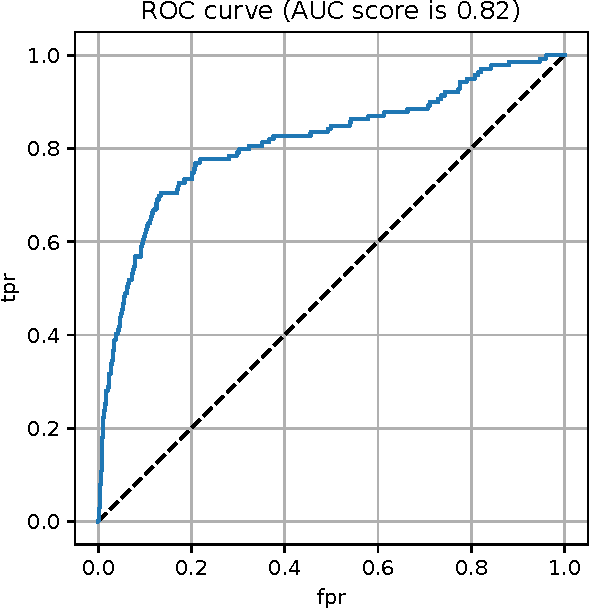
\includegraphics[width=0.35\textwidth]{img/curves_roc}
	\caption{ROC curve. $T\kern-.4exP/P\,\corresponds $ true positive rate (TPR) and $F\kern-.4exP/N\,\corresponds$ false positive rate (FPR)}
\end{figure}

\only<1>{
The higher the area under the curve (ROC AUC) the better the classifier.

\question{What does the dashed diagonal line represent?}

}
\only<2>{

\textbf{But} at the end of the day I need to pick an operating point \notesonly{(i.e. one threshold value)}.

\question{What criterion could I use to favor one threshold over another?}
}

\end{frame}

\mode<article>{
- Assign a ``decision cost $\$_{ij}$'' for different classes 
where $\$_{ij}$ denotes the cost of predicting class $C_{i}$ when the true label is $C_{j}$
(cf. lecture slides 1.4)
}

\begin{frame}

What if the proportions in my training set are different from those of the validation/test set? Which metrics are robust to changes in proportions between different splits of the data.\footnote{cf. jupyter notebook on ISIS for a comparison of different metrics under different conditions.}

\slidesonly{\vspace{-2mm}}

\begin{figure}[h]
	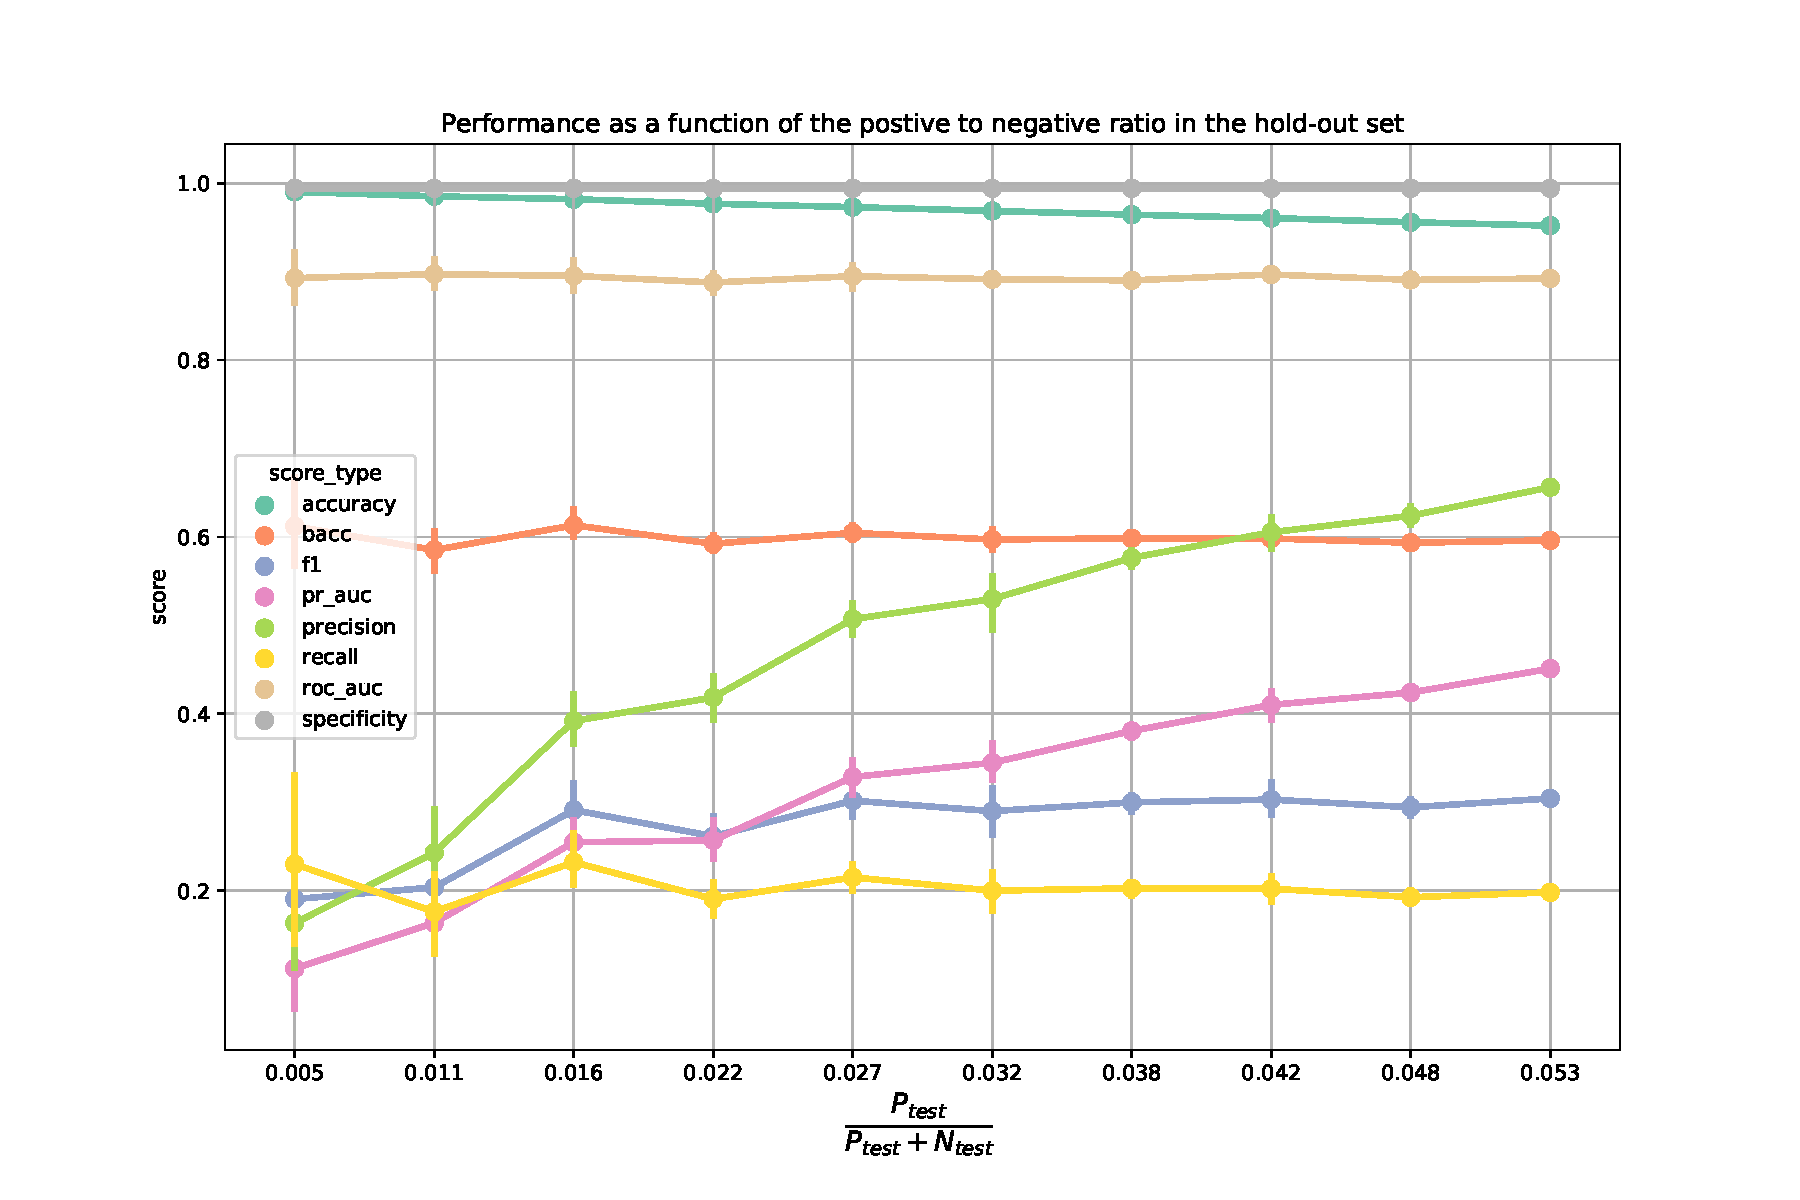
\includegraphics[width=0.8\textwidth]{img/compare_metrics}
	\mode<article>{
	\caption{Comparing metrics under different conditions}
	}
\end{figure}



\end{frame}

\begin{frame}

All we did so far is measure generalization performance and tune our operating point.

\question{Is there anything else we can do about imbalanced data?}

\pause

\begin{enumerate}
\item Train the classifier on a synthetically balanced dataset by
\begin{itemize}
\item sub-sampling from the majority class (no one likes to throw away data)
\item oversampling the minority class
\end{itemize}

\question{Any downsides to oversampling?}

\pause

- the resulting dataset could be too large.
\item class weighted loss function:
e.g. weighted cross entropy:
\begin{equation}
e^{(\alpha)} = -\, \gamma \, y_T^{(\alpha)} \cdot \ln \lbrack y^{(\alpha)} \rbrack - \beta \, (1-y_T^{(\alpha)}) \cdot \ln \lbrack 1-y^{(\alpha)} \rbrack
\end{equation}
where $\beta$ and $\gamma$ represent ``class weights''
\end{enumerate}


\end{frame}




\mode*

\mode<all>
\mode<presentation>{
\begin{frame} 
    \begin{center} \huge
        From Non-parametric classification\\
        to RBF-Networks
    \end{center}
\end{frame}
}

\section{Non-parametric classification}

\subsection{The setting}

\begin{frame}\frametitle{\subsecname~for M-way classification}

\mode<article>{
Specifying the data and model for a multi-class classification with $M$ classes (i.e. $M$-way classification)
}

\begin{itemize}
	\item[]\underline{Data}:
	\begin{equation*}
	\Big\{ \left(\vec x^{(\alpha)}, \vec y^{(\alpha)}_{T} \right) \Big\}_{\alpha=1}^{p}\,
	\end{equation*}

	where $\vec y_T^{(\alpha)} \in \{0, 1\}^M$ with $\sum_{c=1}^{M} (y_{T})_c = 1$ (one-hot encoding of class labels)\\

	\pause

	\item[]\underline{Model}:
	\begin{equation*}
	\vec y(\vec x) \in \R^M 
	\end{equation*}
	with $\sum_{c=1}^{M} y_c(\vec x) = 1$ and $y_c(\vec x)\,\ge\,0\; \forall\,c$\\[2mm]
	
	Predictions $\vec y(\vec x)$ can be used to give
	\begin{itemize}
	\item probabilities of the predicted class (e.g. $y_5(\vec x) = 0.75\; \leadsto$ class ``5'' with 75\% probability.
	\item hard decisions:
    \begin{equation}
    \argmax_{c=1,\ldots,M}\;y_c(\vec x)
    \end{equation}
	\end{itemize}

\end{itemize}

\end{frame}

\subsection{k nearest neighbor classifier}

\begin{frame}\frametitle{\subsecname}
Prediction follows an \emph{electoral committee}; the majority vote of the $k$ nearest neighbors around the query point.

\begin{figure}[h]
	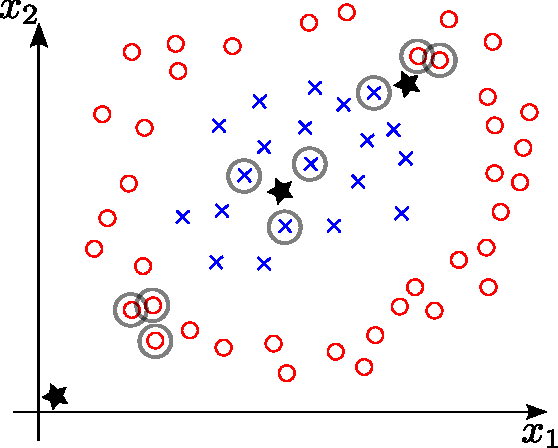
\includegraphics[width=0.3\textwidth]{img/knn}
	\mode<article>{
	\caption{$k$NN with $k=3$}
	}
\end{figure}

Let $k$NN$(\vec x)$ be the indices $\{\beta_1, \beta_2,\ldots,\beta_k\}$ of the $k$ data points closest to $\vec x$ w.r.t. Euclidean norm:

\begin{equation}
\beta_j = 
\argmin_{\substack{\kern-2ex \alpha \in \{1,\ldots,p\} \,\textbackslash\\ \{\beta_{1},\ldots,\beta_{j-1}\}}}
\lVert \vec x^{(\alpha)} \kern-.8ex - \vec x\rVert_{2}
\end{equation}

\end{frame}

\subsubsection{For multi-class classification}

\begin{frame}\frametitle{\subsubsecname}

For multi-class classification the $k$NN classifier (for fixed $k~\corresponds$ hyper-parameter) is defined by:

\begin{equation}
\vec y(\vec x) = \frac{1}{k} \sum_{\beta \in k\mathrm{NN}(\vec x)} \kern-0.5ex \vec y_{T}^{(\beta)}
\label{eq:knn_classifier}
\end{equation}

$\vec y(\vec x)$ \notesonly{in \eqref{eq:knn_classifier}} is effectively an arithmetic average of the labels in the neighborhood.

\end{frame}

\begin{frame}
Example k=3, M=4

\begin{equation}
\vec y(\vec x) = \frac{1}{3}
\left\lbrack
\,
\rmat{ 1 \\ 0 \\ 0 \\ 0}\, +\,
\rmat{ 1 \\ 0 \\ 0 \\ 0} +\,
\rmat{ 0 \\ 1 \\ 0 \\ 0}\,
\right\rbrack
=
\frac{1}{3}
\rmat{ 2 \\ 1 \\ 0 \\ 0}
=
\rmat{ 2/3 \\ 1/3 \\ 0\; \\ 0\;}
\end{equation}

applying a hard decision would yield $c=1$.
    
\end{frame}

\subsubsection{the binary classification case}

\begin{frame}\frametitle{\subsubsecname}

For binary classification, we can set $M=2$ for a multi-class $k$NN classifier.

Alternatively, we can construct the $k$NN classifier \notesonly{for binary classification} using \emph{scalar} labels:

\begin{equation}
y_T \in \{0,1\}\quad \text{ and }\quad y(\vec x) \in \R
\end{equation}
with

\begin{equation}
y(\vec x) \ge\,0\,:\,
\begin{cases*}
      \;y(\vec x) & probability of class $1$ \\
      \;1-y(\vec x)     & probability of class $0$
    \end{cases*}
\end{equation}

\end{frame}

\begin{frame}

\question{What is the role of $k$ in terms of model complexity? $k = 1$ vs. $k = p$}

\mode<presentation>{

\begin{figure}[h]
	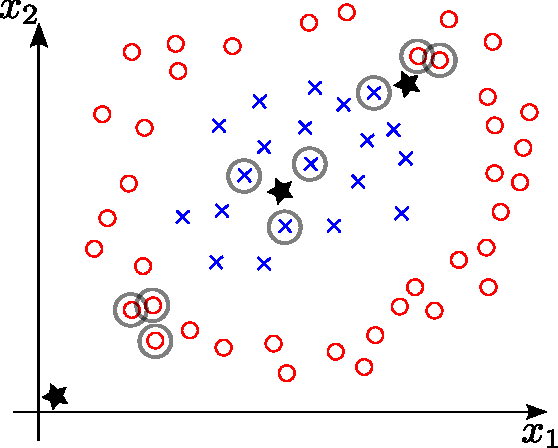
\includegraphics[width=0.4\textwidth]{img/knn}
	\mode<article>{
	\caption{$k$NN with $k=3$}
	}
\end{figure}

}

\pause

\question{How would you select the $k$ nearest neighbors for some query point $\vec x$?}

\pause

Hint: Jitter the data (or the query points) and see which choice of $k$ leads to different (more noisy) predictions.

\mode<article>{

Remarks:
\begin{enumerate}
\item The value of $k$ controls the model complexity ($k = 1 \leadsto$ over-fitting, larger $k \leadsto$ under-fitting)

\item Selecting the $k$ nearest neighbors of some point $\vec x$ can be costly but can be made more efficient using data structures such as \emph{Kdtrees})
\end{enumerate}
}

\end{frame}

\mode*

\clearpage

\mode<all>
\subsection{Parzen window classification}

\mode<presentation>{
\begin{frame} 
    \begin{center} \huge
        \subsecname
    \end{center}
    \begin{center}
    
\includegraphics[width=0.4\textwidth]{img/meme_wow_parzen}
    \end{center}
    \begin{center}
    $k$NN with all points, but weighted by a window.
    \end{center}
\end{frame}
}


\begin{frame}\frametitle{\subsecname}

Prediction is based on 
\begin{itemize}
\item \underline{all} data points \notesonly{(no longer restricted to the $k$ nearest neighbors)}
\item \notesonly{and the contribution of each point is} weighted according to some window/``kernel'' function $\kappa(\vec x, \vec x')$ \notesonly{evaluated for a pair of points $\vec x$ and $\vec x'$}.
\end{itemize}

\begin{equation}
\vec y(\vec x) := \frac{1}{Z} \sum_{\alpha=1}^{p}\;\vec y_T^{(\alpha)} \kappa(\vec x, \vec x^{(\alpha)})
\end{equation}

with

\begin{equation}
Z := \sum_{\alpha=1}^{p} \kappa(\vec x, \vec x^{(\alpha)})
\end{equation}

\end{frame}

\begin{frame}{The Gaussian kernel}

An example for the window/``kernel'' function $\kappa(\vec x, \vec x')$ would be the Gaussian function:

\begin{equation}
\kappa(\vec x, \vec x') := \exp\left( -\,\frac{\lVert \vec x - \vec x'\rVert^2_2}{2\,\sigma_{\kappa}^2} \right)
\label{eq:gauss_kernel}
\end{equation}

where $\sigma_{\kappa}$ is referred to as the \emph{width} of the kernel.

\begin{figure}[ht]
     \centering
     \savebox{\imagebox}{
	 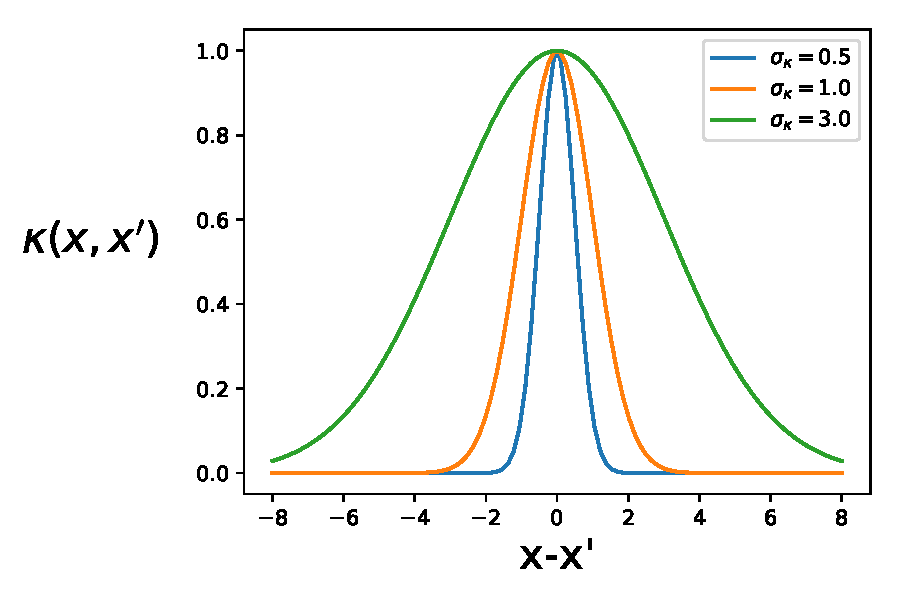
\includegraphics[width=0.45\textwidth]{img/guassian_function_1d}}%
     \begin{subfigure}[t]{0.45\textwidth}
         \centering
         \usebox{\imagebox}% Place largest image
         \caption{For data in 1D}
         \label{fig:quadratic}
     \end{subfigure}
     \hspace{2mm}
     \begin{subfigure}[t]{0.45\textwidth}
         \centering
         \raisebox{\dimexpr.5\ht\imagebox-.5\height}{% Raise smaller image into place
         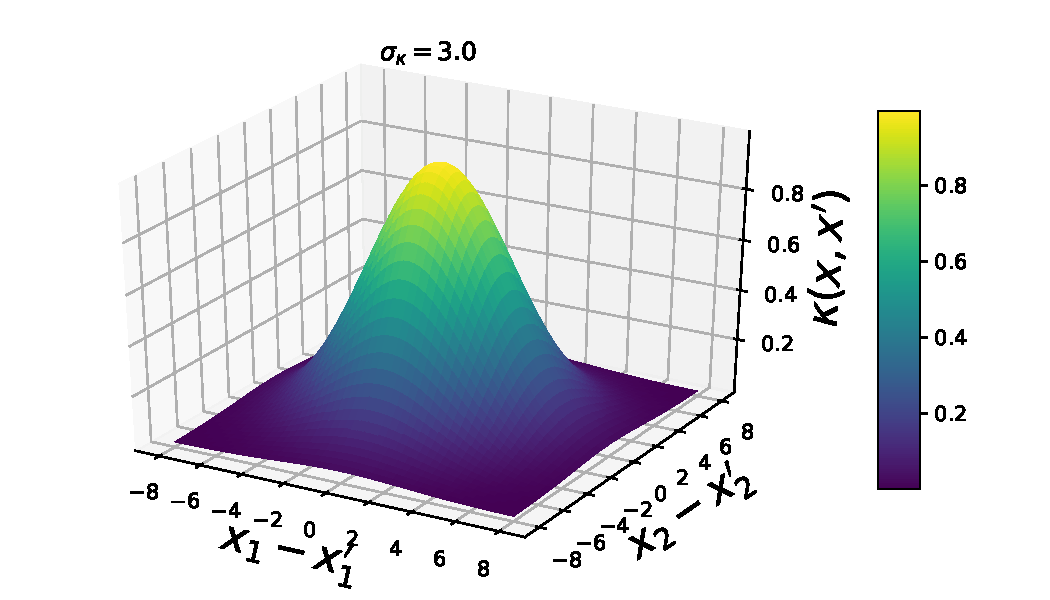
\includegraphics[width=0.99\textwidth]{img/guassian_function_2d_3Dview}
         }
         \caption{For data in 2D}
         \label{fig:linear}
     \end{subfigure}
     \mode<article>{
     \caption{The Gaussian kernel function}
     }
	 \label{fig:quadratic_density_gaussian}
\end{figure}

\end{frame}

\begin{frame}{Binary classification example with 2D data}

\notesonly{
Binary classification example with 2D data:
}

\begin{figure}[ht]
     \centering
     \savebox{\imagebox}{
	 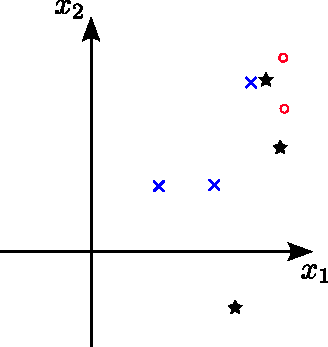
\includegraphics[width=0.3\textwidth]{img/parzen_data}}%
     \begin{subfigure}[t]{0.3\textwidth}
         \centering
         \usebox{\imagebox}% Place largest image
         \caption{Binary classification data in 2D}
     \end{subfigure}
     \hspace{2mm}
     \visible<2>{
     \begin{subfigure}[t]{0.3\textwidth}
         \centering
         \raisebox{\dimexpr.5\ht\imagebox-.5\height}{% Raise smaller image into place
         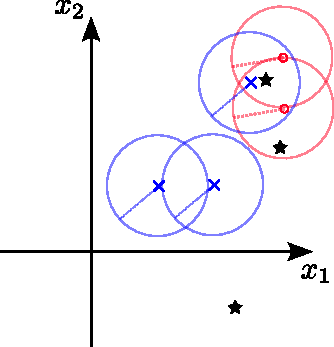
\includegraphics[width=0.99\textwidth]{img/parzen_circles}
         }
         \notesonly{
         \caption{A Gaussian window around each training point}
         }
     \end{subfigure}
     }
\end{figure}


\mode<presentation>{

\begin{equation}
\vec y(\vec x) := \frac{1}{Z} \sum_{\alpha=1}^{p} \vec y_T^{(\alpha)} \, \kappa(\vec x, \vec x^{(\alpha)})
\end{equation}

\begin{equation}
\kappa(\vec x, \vec x^{(\alpha)}) := \exp\left( -\,\frac{\lVert \vec x - \vec x^{(\alpha)}\rVert^2_2}{2\,\sigma_{\kappa}^2} \right)
\label{eq:gauss_kernel}
\end{equation}

}

\end{frame}

\begin{frame}

\begin{figure}[ht]
     \centering
     \savebox{\imagebox}{
	 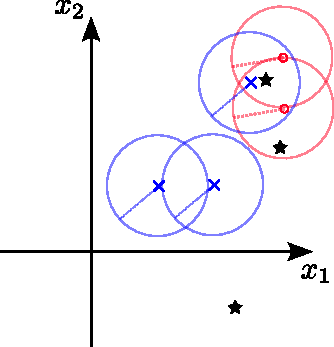
\includegraphics[width=0.37\textwidth]{img/parzen_circles}}%
     \begin{subfigure}[t]{0.37\textwidth}
         \centering
         \usebox{\imagebox}% Place largest image
         \caption{wide kernel width}
         \label{fig:quadratic}
     \end{subfigure}
     \hspace{2mm}
     \begin{subfigure}[t]{0.37\textwidth}
         \centering
         \raisebox{\dimexpr.5\ht\imagebox-.5\height}{% Raise smaller image into place
         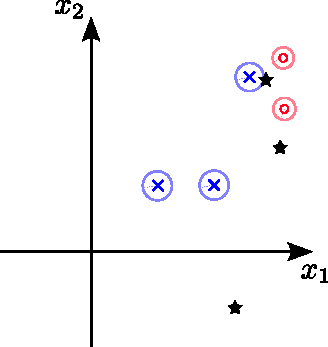
\includegraphics[width=0.99\textwidth]{img/parzen_circles_narrow}
         }
         \caption{narrow kernel width}
         \label{fig:linear}
     \end{subfigure}
\end{figure}

\question{What is the role of the kernel width $\sigma_{\kappa}$ in terms of model complexity?}

\pause

Hint: Jitter the query points (or the data) and see which choice of $\sigma_{\kappa}$ will lead to different (more noisy) predictions.

\end{frame}

\begin{frame}

Remarks:
\begin{enumerate} 
\item The width of the kernel $\kappa$ controls the model complexity (narrow width $\leadsto$ over-fitting (high variance), wide $\leadsto$ under-fitting)
 
One way to go about this is to apply a small noise to the query points (i.e. jitter) and see how the predictions will vary with different $\sigma_{\kappa}$. If this small noise in the position of the points leads to different predictions we are basically looking at high variance.

\item Using all data points. Potentially costly with large $p$
\end{enumerate}
\end{frame}

\mode*

\clearpage

\mode<all>


\section{RBF-Networks}

\mode<presentation>{
\begin{frame} 
    \begin{center} \huge
        \secname
    \end{center}
    \begin{center}
    
\includegraphics[width=0.4\textwidth]{img/meme_wow_rbf}
    \end{center}
    \begin{center}
    Parzen window classification with ``representatives''
    \end{center}
\end{frame}
}

\begin{frame}\frametitle{\secname}

A trade-off between $k$NN classification and Parzen window classification.

Instead of taking all $p$ points to predict the class probabilities (Parzen), limit the prediction to $k \ll p$ \cancel{points} ``representative'' functions.

Represent all points $\vec x$ in terms of basis functions $\phi_i(\vec x), i=1\,\ldots,k$

Let $k$ be the number of basis functions.

\end{frame}

\begin{frame}

\begin{figure}[ht]
     \centering
     \savebox{\imagebox}{
	 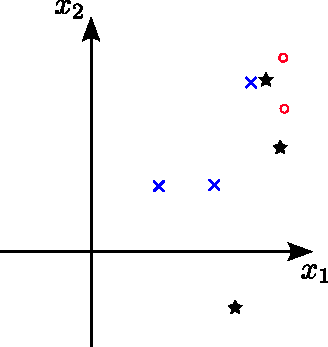
\includegraphics[width=0.34\textwidth]{img/parzen_data}}%
     \begin{subfigure}[t]{0.37\textwidth}
         \centering
         \usebox{\imagebox}% Place largest image
         \caption{Two-class data in 2D}
         \label{fig:quadratic}
     \end{subfigure}
     \hspace{2mm}
     \begin{subfigure}[t]{0.37\textwidth}
         \centering
         \raisebox{\dimexpr.5\ht\imagebox-.5\height}{% Raise smaller image into place
         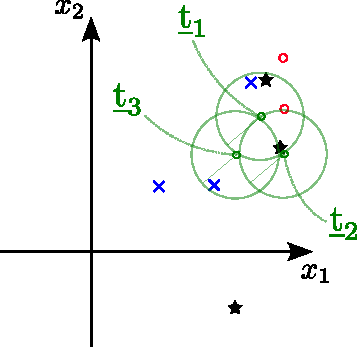
\includegraphics[width=0.99\textwidth]{img/rbf-network}
         }
         \caption{$k=3$ ``representatives''}
         \label{fig:rbf-network}
     \end{subfigure}
\end{figure}

\end{frame}

\subsection{Recap: Regression on transformed data using nonlinear basis functions}


\subsection{Nonlinear basis function}


\begin{frame}\frametitle{\subsecname}

Feature transformation $(\vec x\in \R^N)$:

\begin{equation}
\vec \phi: \vec x \mapsto \vec \phi(\vec x)
\end{equation}

\mode<article>{$\phi(\vec x)$ can transform our $N$-dim input $\vec x$ into the feature space spanned by the $k$ basis functions positioned at $\vec t_1,\ldots,\vec t_k$.
}

Assume $\{\vec t_i\}$ and corresponding kernel width $\{\sigma_i\}$ have already been determined.

Transform the feature space using \emph{radial basis functions} (Gaussian kernel functions):

\begin{align}
\phi_i(\vec x) \in 
\exp\left( -\,\frac{\lVert \vec x - \vec t_i\rVert^2_2}{2\,\sigma_{i}^2} \right), \quad i=1,\ldots,k
\end{align}

\end{frame}

\subsection{Setting for binary classification/ scalar regression}

\begin{frame}\frametitle{\subsecname}

\underline{Data}:\\

\begin{table}[h]
\begin{tabular}{rl}
transformed input & $\vec \phi^{(\alpha)} := \vec \phi(\vec x^{(\alpha)}) = \big ( 
\underbrace{1}_{\phi_{0}},
\phi_{1}(\vec x^{(\alpha)}), \ldots, \phi_{k}(\vec x^{(\alpha)}) \big)^{\top}$\\
&$\Rightarrow \vec \phi^{(\alpha)} \in \R^{k+1}$ \\[2mm]
label         & $y_{T}^{(\alpha)} \in \R$ \\
with & $\alpha = 1,\ldots,p$
\end{tabular}
\end{table}

\end{frame}

\begin{frame}\frametitle{\subsecname}

\underline{Model}:
\vspace{-5mm}
\only<1>{
	\begin{center}
		\raisebox{-3.35cm}{\includegraphics[height=5.25cm]%
			{img/section1_fig38_v2} }
		$ = \sum\limits_i \mathrm{w}_i \phi_i(\vec{x})$
	\end{center}
}
\vspace{-5mm}
\notesonly{The output is a linear neuron on the \emph{the transformed} input:}

\begin{equation}
    y(\vec \phi; \vec w) = \sum_{i=0}^{k} w_{i} \phi_{i}(\vec x) = \vec w^{\top} \vec \phi
\end{equation}

\notesonly{
Start from $i=0$ to include bias node (unlike the case with monomials where the bias was already present at $i=1$).
}
\slidesonly{Don't forget the bias!
}
Set $\vec \Phi = \left( \vec \phi^{(1)},\ldots, \vec \phi^{(\alpha)},\ldots, \vec \phi^{(p)}\right) \in \R^{k+1,p}$

quadratic cost function. \pause Reuse solution for linear regression:

\begin{equation}
\vec w^{*} = \left( \vec \Phi \, \vec \Phi^{\top}\right)^{-1} \vec \Phi \, \vec y_{\text{True}}^{\top}
\end{equation}

\question{What about using RBF-Networks for classification?}

\pause

- The quadratic cost function can still be applied to learning the parameters in an RBF-Network for solving classification problems as well but the performance is often less than when using cross-entropy loss.

\end{frame}

\subsection{Multi-dimensional RBF-Networks}

\begin{frame}\frametitle{\subsecname}

Generalizing nonlinear basis functions in linear models:

\begin{equation}
\vec y(\vec \phi(\vec x)) = 
\rmat{
y_1(\vec \phi(\vec x))\\
y_2(\vec \phi(\vec x))\\
\vdots\qquad\\
y_M(\vec \phi(\vec x))
}
= \vec W^\top \kern-.5ex \vec \phi(\vec x)
\end{equation}

\svspace{-3mm}

with $\vec W \in \R^{k+1,M}$

closed form solution for quadratic cost: 

\begin{equation}
\vec W^{*} =
\underbrace{
\left(\vec \Phi \, \vec \Phi^{\top} \right)^{-1}
}_{
\substack{
\text{assume}\\ \text{invertibility}}
}
\vec \Phi \, \vec Y_{\text{True}}^{\top}
\end{equation}

\question{What is $\vec Y_{\text{True}}$? What is the shape of this matrix?}

\pause

\svspace{-3mm}

\notesonly{where} $\vec Y_{\text{True}} := \left( \vec y_{\text{True}}^{(1)},\ldots,\vec y_{\text{True}}^{(p)}\right) \in \R^{M,p}$

\end{frame}

\begin{frame}
Remarks:

\begin{itemize}
\item RBF-Networks are universal function approximators like MLPs.
\item RBF-Networks suffer from the ``curse of dimensionality''
\item Regularization is needed:

For weight decay:
\begin{equation}
\vec W^{*} = \left( \vec \Phi \, \vec \Phi^{\top} + \lambda\,\vec I_{k+1} \,\right)^{-1} \vec \Phi \, \vec Y_{\text{True}}^{\top}
\end{equation}

\end{itemize}

\end{frame}

\subsection{RBF-Network vs. Parzen window classification}

\begin{frame}\frametitle{\subsecname}

\mode<presentation>{
\begin{equation}
\vec y_{\text{Parzen}}(\vec x) := \frac{1}{Z} \sum_{\alpha=1}^{p} \vec y_T^{(\alpha)}\, \kappa(\vec x, \vec x^{(\alpha)})
\qquad \text{(Parzen window classifier)}
\end{equation}
\begin{equation}
    \vec y_{\text{RBF-Net}}(\vec \phi; \vec w) = \sum_{i=0}^{k} w_{i} \phi_{i}(\vec x) \qquad \text{(RBF-Network)}
\end{equation}
}

\question{Which model class is a generalization of the other?}

\pause 

\svspace{-3mm}

\question{How would you construct an RBF-Network to mimic a Parzen window classifier?}

\pause

- An RBF-Network can be constructed and parameterized to act as a Parzen window classifier by placing a ``representative'/centroid over every point $^{(\alpha)}$.





\end{frame}

\begin{frame}

\question{Can an RBF-Network solve this problem? How?}

	\begin{center}
		\raisebox{-3.35cm}{\includegraphics[height=5.25cm]%
			{img/circular} }
	\end{center}

\end{frame}

\begin{frame}

\question{Can an RBF-Network solve this problem? How many basis functions does it need?}

	\begin{center}
		\raisebox{-3.35cm}{\includegraphics[height=5.25cm]%
			{img/sdata} }
	\end{center}

\end{frame}

\begin{frame}

\question{Can an RBF-Network solve this problem using only 2 centroids?}

	\begin{center}
		\raisebox{-3.35cm}{\includegraphics[height=5.25cm]%
			{img/circular_3classes_v2} }
	\end{center}

\end{frame}

\newpage

\subsection{MLPs vs. RBF-Networks}

\notesonly{cf. Haykin 5.11}

\begin{frame}

\slidesonly{\vspace{-2mm}
}
{
\slidesonly{\footnotesize}
\begin{table}[h]
\begin{tabular}{|l|l|}
\hline
\multicolumn{1}{|c|}{MLPs}                                                                          & \multicolumn{1}{c|}{RBF-Networks}                                                                                                      \\ 



\hline\pause

global approximation                                                                                &                                                                                          \begin{tabular}[c]{@{}l@{}}local approximation\\due to exponentially decaying non-linearity\end{tabular}                            \\ 
\hline\pause

\begin{tabular}[c]{@{}l@{}}+ better performance than RBF \\ with same \# of parameters\end{tabular} & \begin{tabular}[c]{@{}l@{}}- less performance than MLP \\ with same \# of parameters\end{tabular}                                      \\ 
\hline\pause

\begin{tabular}[c]{@{}l@{}}+ usually better performance\\ with larger datasets\end{tabular}         & + suitable for small datasets                                                                                                          \\ 
\hline\pause

- data hungry                                                                                       & \begin{tabular}[c]{@{}l@{}}+ faster training with \\ small \# of basis functions\end{tabular}                                          \\ 
\hline\pause

+ adapts functions to data and labels                                                               & \begin{tabular}[c]{@{}l@{}}can benefit from unlabeled data\\ (semi-supervised learning)\end{tabular}                                   \\ 
\hline\pause

\begin{tabular}[c]{@{}l@{}}common neuronal mode \\between hidden and output neurons\end{tabular}                  & \begin{tabular}[c]{@{}l@{}}The hidden layer serves a \\very different purpose\\than the output layer\end{tabular} \\ 
\hline\pause

\begin{tabular}[c]{@{}l@{}}total input of a hidden neuron\\determined via inner product\\$\vec w_i^\top \vec x$\end{tabular}                  & \begin{tabular}[c]{@{}l@{}}total input is based on a Euclidean distance\end{tabular} \\ 
\hline\pause

\begin{tabular}[c]{@{}l@{}}\end{tabular}                  & \begin{tabular}[c]{@{}l@{}}restricted function class (many \\ basis functions needed\\ for complicated approximations)\end{tabular} \\ 
\hline\pause

\begin{tabular}[c]{@{}l@{}}\end{tabular}                             & \begin{tabular}[c]{@{}l@{}}benefits from clustered structure\\ in the data\end{tabular}                                                \\ \hline
\end{tabular}
\end{table}
}

\end{frame}


\mode*

\clearpage


\end{rightcolumn}
\end{paracol}

\end{document}
